Prin natura distribuita a crawler-ului "Surf", acesta asigura viteza in parcurgerea paginilor web si un grad crescut de redundanta in vederea extragerii informatiilor din sursele selectate. Scalabilitatea orizontala\footnote{\textit{"scalabilitatea orizontala"} reprezinta posibilitatea de a adauga mai multe masini de lucru unui sistem informatic, pentru a ii mari performanta} si verticala\footnote{\textit{"scalabilitatea verticala"} se refera la posibilitatea de a imbunatati performanta masinilor de calcul dintr-un sistem informatic, prin adaugarea de hardware mai performant} este garantata de mecanismele de scalare ale serviciilor web din cadrul Amazon Web Services.
\\ 

Fie ca este vorba despre API-ul "Surf", mecanismul asincron de notificari (SNS), asigurarea spatiului de stocare (S3) sau functiile Lambda (centrul computational al crawler-ului "Surf"), efortul utilizatorului pentru a ajusta performanta sistemelor mentionate consta doar in a ajusta configurarile corespunzatoare serviciului care se doreste a fi scalat\footnote{un serviciu web poate fi scalat atat in sus, adaugand putere computationala, cat si in jos, renuntand la putere de calcul}. In consecinta, costurile vor varia in functie de gradul de performanta care se doreste a fi atins. Graficele de mai jos (\textit{"Figura 9"} si \textit{"Figura 10"}) prezinta comparatii relative intre o serie variata de configurari ale sistemului cloud ce gazduieste aplicatia "Surf". \textit{"Figura 9"} are in vedere configuratia \textit{"adancime maxima: 5, numar maxim de pagini pe nivel: 30, timp de terminare sarcini maxim pentru workeri: 40 secunde, adresa de pornire: http://news.ycombinator.com/news"}. \textit{"Figura 10"} este diferita prin faptul ca prezinta configuratia \textit{"adancime maxima: 3, numar maxim de pagini pe nivel: 100"}.
\\

Din diagramele din figurile 9 si 10 se poate observa faptul ca gradul de paralelizare are un impact direct asupra performantei crawler-ului. Testele s-au realizat atunci cand sistemul nu prezenta incarcatura (i.e. task-uri in executare) din alte motive decat cele in scopul determinarii performantei crawler-ului. Desi este de asteptat ca performanta sa se degradeze odata ce mai multi utilizatori incep sa foloseasca serviciul de crawling "Surf", pierderea de performanta se poate compensa crescand cantitatea de resurse alocate pentru fiecare functie Lambda (i.e. procesor si memorie) si prin configurarea tabelelor DynamoDB in vederea acceptarii unui numar mai mare de cereri pe secunda.

\begin{figure}[ht]
\begin{center}
	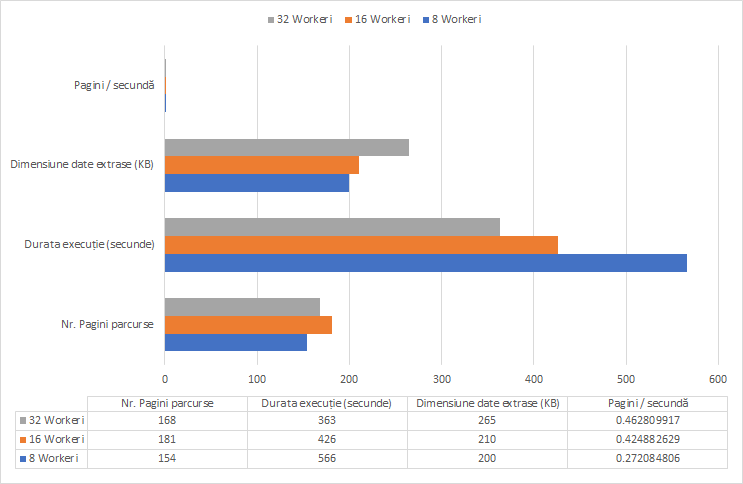
\includegraphics[keepaspectratio, width=0.9\textwidth]{depth-performance-chart.png}
	\caption{Performanta crawler-ului "Surf" la parcurgerile in adancime \cite{diagram-icons-sources, aws-icons-source, microsoft-excel}}\par\medskip 

\end{center}
\end{figure}

\begin{figure}[ht]
\begin{center}
	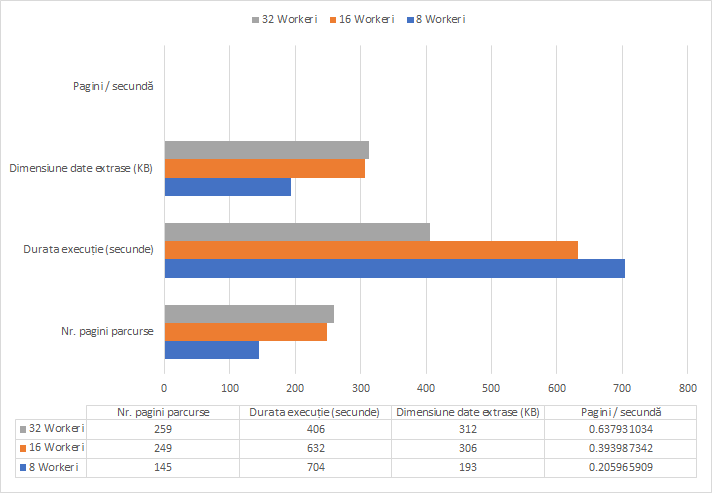
\includegraphics[keepaspectratio, width=0.9\textwidth]{breadth-performance-chart.png}
	\caption{Performanta crawler-ului "Surf" la parcurgerile pe niveluri \cite{diagram-icons-sources, aws-icons-source, microsoft-excel}}\par\medskip 

\end{center}
\end{figure}

